\documentclass[border=15pt]{standalone}
\usepackage{tikz}
\usepackage{amsmath,amssymb}
\usepackage{xcolor}
\usetikzlibrary{shapes,arrows.meta,positioning,shadows,calc,fit,backgrounds}

% Define clean, academic colors (Nature / NeurIPS style)
\definecolor{darkslate}{HTML}{0F172A}
\definecolor{blueborder}{HTML}{2563EB}
\definecolor{bluefill}{HTML}{EFF6FF}
\definecolor{bluehead}{HTML}{1E40AF}

\definecolor{tealborder}{HTML}{0D9488}
\definecolor{tealfill}{HTML}{F0FDFA}
\definecolor{tealhead}{HTML}{0F766E}

\definecolor{purpleborder}{HTML}{9333EA}
\definecolor{purplefill}{HTML}{FAF5FF}
\definecolor{purplehead}{HTML}{6B21A8}

\definecolor{greenborder}{HTML}{16A34A}
\definecolor{greenfill}{HTML}{F0FDF4}
\definecolor{greenhead}{HTML}{15803D}

\definecolor{redborder}{HTML}{E11D48}
\definecolor{redfill}{HTML}{FFF1F2}
\definecolor{redhead}{HTML}{9F1239}

\begin{document}
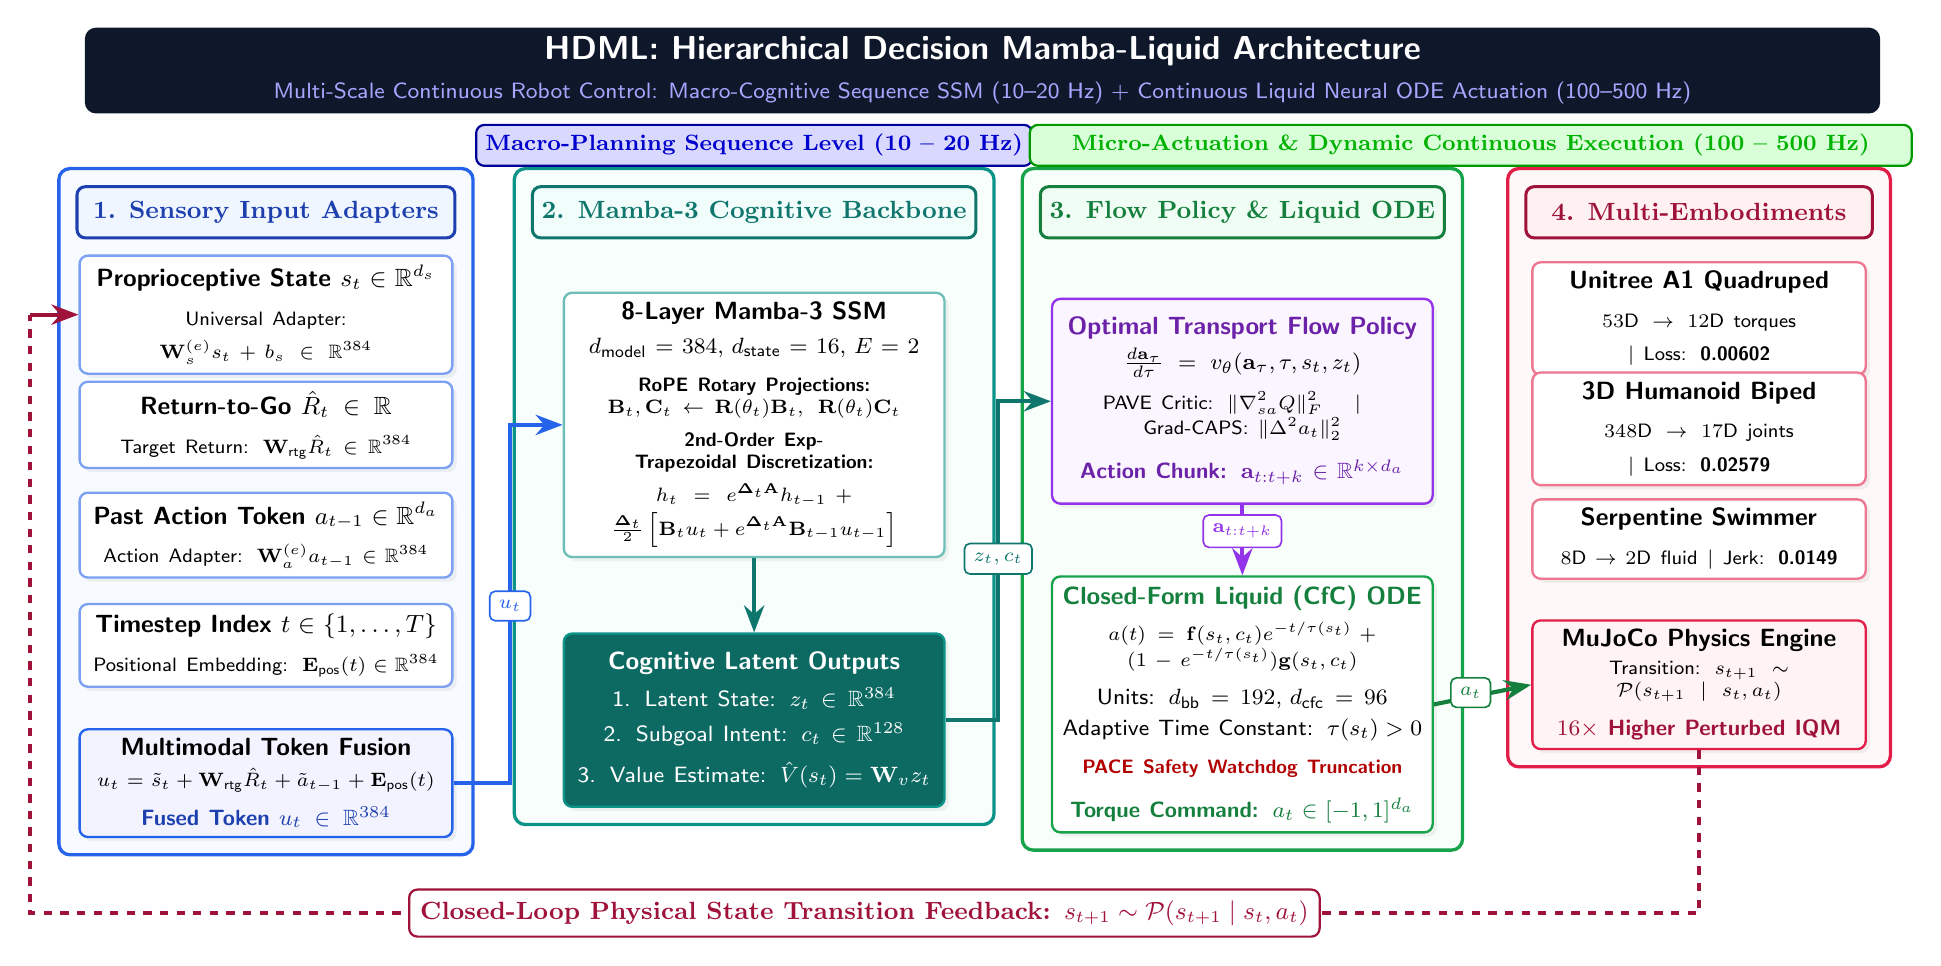
\begin{tikzpicture}[
    font=\sffamily,
    >=Stealth,
    headerbase/.style={
        rectangle, rounded corners=3pt, line width=1.1pt,
        minimum height=0.65cm, align=center, font=\bfseries\small
    },
    boxbase/.style={
        rectangle, rounded corners=3pt, line width=0.85pt,
        align=center, drop shadow={opacity=0.10, shadow xshift=1.5pt, shadow yshift=-1.5pt}
    },
    arrowstyle/.style={
        ->, line width=1.5pt, draw=#1
    }
]

% =========================================================================
% TOP HEADER & TIMESCALES
% =========================================================================
\node[rectangle, rounded corners=4pt, fill=darkslate, text=white, minimum width=22.8cm, minimum height=1.05cm, align=center] at (9.1, 10.3) {
    {\large \textbf{HDML: Hierarchical Decision Mamba-Liquid Architecture}}\\[2pt]
    {\footnotesize \color{blue!35} Multi-Scale Continuous Robot Control: Macro-Cognitive Sequence SSM (10--20 Hz) + Continuous Liquid Neural ODE Actuation (100--500 Hz)}
};

\node[rectangle, rounded corners=3pt, fill=blue!15, draw=blue!60!black, line width=0.8pt, minimum width=5.2cm, minimum height=0.52cm, font=\bfseries\footnotesize, text=blue!80!black] at (6.2, 9.35) {
    Macro-Planning Sequence Level (10 -- 20 Hz)
};

\node[rectangle, rounded corners=3pt, fill=green!15, draw=green!60!black, line width=0.8pt, minimum width=11.2cm, minimum height=0.52cm, font=\bfseries\footnotesize, text=green!70!black] at (15.3, 9.35) {
    Micro-Actuation \& Dynamic Continuous Execution (100 -- 500 Hz)
};

% =========================================================================
% COLUMN 1: SENSORY INPUT ADAPTERS (Center x = 0.0)
% =========================================================================
\node[headerbase, draw=bluehead, fill=bluefill, text=bluehead, minimum width=4.8cm] (h1) at (0.0, 8.5) {1. Sensory Input Adapters};

\node[boxbase, draw=blueborder!60, fill=white, text width=4.5cm, minimum height=1.05cm] (b_s) at (0.0, 7.2) {
    \textbf{\small Proprioceptive State $s_t \in \mathbb{R}^{d_s}$}\\[2pt]
    \scriptsize Universal Adapter: $\mathbf{W}_s^{(e)} s_t + b_s \in \mathbb{R}^{384}$
};

\node[boxbase, draw=blueborder!60, fill=white, text width=4.5cm, minimum height=1.05cm] (b_r) at (0.0, 5.8) {
    \textbf{\small Return-to-Go $\hat{R}_t \in \mathbb{R}$}\\[2pt]
    \scriptsize Target Return: $\mathbf{W}_{\text{rtg}} \hat{R}_t \in \mathbb{R}^{384}$
};

\node[boxbase, draw=blueborder!60, fill=white, text width=4.5cm, minimum height=1.05cm] (b_a) at (0.0, 4.4) {
    \textbf{\small Past Action Token $a_{t-1} \in \mathbb{R}^{d_a}$}\\[2pt]
    \scriptsize Action Adapter: $\mathbf{W}_a^{(e)} a_{t-1} \in \mathbb{R}^{384}$
};

\node[boxbase, draw=blueborder!60, fill=white, text width=4.5cm, minimum height=1.05cm] (b_pos) at (0.0, 3.0) {
    \textbf{\small Timestep Index $t \in \{1,\dots,T\}$}\\[2pt]
    \scriptsize Positional Embedding: $\mathbf{E}_{\text{pos}}(t) \in \mathbb{R}^{384}$
};

\node[boxbase, draw=blueborder, fill=bluefill!80!blue!20, text width=4.5cm, minimum height=1.3cm] (b_fuse) at (0.0, 1.25) {
    \textbf{\small Multimodal Token Fusion}\\[3pt]
    \scriptsize $u_t = \tilde{s}_t + \mathbf{W}_{\text{rtg}}\hat{R}_t + \tilde{a}_{t-1} + \mathbf{E}_{\text{pos}}(t)$\\[2pt]
    \footnotesize \textbf{\color{bluehead} Fused Token $u_t \in \mathbb{R}^{384}$}
};

% Column 1 Background Box
\begin{scope}[on background layer]
\node[rectangle, rounded corners=4pt, draw=blueborder, line width=1.2pt, fill=bluefill!50,
      fit={(h1) (b_s) (b_fuse)}, inner sep=6pt] (col1_bg) {};
\end{scope}

% =========================================================================
% COLUMN 2: MAMBA-3 COGNITIVE BACKBONE (Center x = 6.2)
% =========================================================================
\node[headerbase, draw=tealhead, fill=tealfill, text=tealhead, minimum width=5.0cm] (h2) at (6.2, 8.5) {2. Mamba-3 Cognitive Backbone};

\node[boxbase, draw=tealborder!60, fill=white, text width=4.6cm, minimum height=3.3cm] (b_mamba) at (6.2, 5.8) {
    \textbf{\small 8-Layer Mamba-3 SSM}\\[3pt]
    \footnotesize $d_{\text{model}} = 384, \, d_{\text{state}} = 16, \, E = 2$\\[4pt]
    \textbf{\scriptsize RoPE Rotary Projections:}\\
    \scriptsize $\mathbf{B}_t, \mathbf{C}_t \leftarrow \mathbf{R}(\theta_t)\mathbf{B}_t, \; \mathbf{R}(\theta_t)\mathbf{C}_t$\\[4pt]
    \textbf{\scriptsize 2nd-Order Exp-Trapezoidal Discretization:}\\
    \scriptsize $h_t = e^{\mathbf{\Delta}_t \mathbf{A}}h_{t-1} + \frac{\mathbf{\Delta}_t}{2}\left[\mathbf{B}_t u_t + e^{\mathbf{\Delta}_t \mathbf{A}}\mathbf{B}_{t-1}u_{t-1}\right]$
};

\node[boxbase, draw=tealborder, fill=tealhead!90!black, text width=4.6cm, minimum height=2.2cm, text=white] (b_latent) at (6.2, 2.05) {
    \textbf{\small Cognitive Latent Outputs}\\[4pt]
    \footnotesize 1. Latent State: $z_t \in \mathbb{R}^{384}$\\[3pt]
    \footnotesize 2. Subgoal Intent: $c_t \in \mathbb{R}^{128}$\\[3pt]
    \footnotesize 3. Value Estimate: $\hat{V}(s_t) = \mathbf{W}_v z_t$
};

% Column 2 Background Box
\begin{scope}[on background layer]
\node[rectangle, rounded corners=4pt, draw=tealborder, line width=1.2pt, fill=tealfill!50,
      fit={(h2) (b_mamba) (b_latent)}, inner sep=6pt] (col2_bg) {};
\end{scope}

% =========================================================================
% COLUMN 3: FLOW POLICY & LIQUID CFC ODE (Center x = 12.4)
% =========================================================================
\node[headerbase, draw=greenhead, fill=greenfill, text=greenhead, minimum width=5.0cm] (h3) at (12.4, 8.5) {3. Flow Policy \& Liquid ODE};

\node[boxbase, draw=purpleborder, fill=purplefill, text width=4.6cm, minimum height=2.6cm] (b_flow) at (12.4, 6.1) {
    \textbf{\small \color{purplehead} Optimal Transport Flow Policy}\\[3pt]
    \footnotesize $\frac{d\mathbf{a}_\tau}{d\tau} = v_\theta(\mathbf{a}_\tau, \tau, s_t, z_t)$\\[4pt]
    \scriptsize PAVE Critic: $\|\nabla_{sa}^2 Q\|_F^2 \quad \mid \quad$ Grad-CAPS: $\|\Delta^2 a_t\|_2^2$\\[4pt]
    \footnotesize \textbf{\color{purplehead} Action Chunk: $\mathbf{a}_{t:t+k} \in \mathbb{R}^{k \times d_a}$}
};

\node[boxbase, draw=greenborder, fill=white, text width=4.6cm, minimum height=2.9cm] (b_cfc) at (12.4, 2.25) {
    \textbf{\small \color{greenhead} Closed-Form Liquid (CfC) ODE}\\[3pt]
    \scriptsize $a(t) = \mathbf{f}(s_t, c_t) e^{-t/\tau(s_t)} + (1-e^{-t/\tau(s_t)})\mathbf{g}(s_t, c_t)$\\[4pt]
    \footnotesize Units: $d_{\text{bb}}=192, \, d_{\text{cfc}}=96$\\[2pt]
    \footnotesize Adaptive Time Constant: $\tau(s_t) > 0$\\[4pt]
    \textbf{\scriptsize \color{red!70!black} PACE Safety Watchdog Truncation}\\[4pt]
    \footnotesize \textbf{\color{greenhead} Torque Command: $a_t \in [-1, 1]^{d_a}$}
};

% Column 3 Background Box
\begin{scope}[on background layer]
\node[rectangle, rounded corners=4pt, draw=greenborder, line width=1.2pt, fill=greenfill!50,
      fit={(h3) (b_flow) (b_cfc)}, inner sep=6pt] (col3_bg) {};
\end{scope}

% =========================================================================
% COLUMN 4: MULTI-EMBODIMENTS (Center x = 18.2)
% =========================================================================
\node[headerbase, draw=redhead, fill=redfill, text=redhead, minimum width=4.4cm] (h4) at (18.2, 8.5) {4. Multi-Embodiments};

\node[boxbase, draw=redborder!60, fill=white, text width=4.0cm, minimum height=0.95cm] (r_a1) at (18.2, 7.15) {
    \textbf{\small Unitree A1 Quadruped}\\[2pt]
    \scriptsize $53\text{D} \to 12\text{D}$ torques $\mid$ Loss: \textbf{0.00602}
};

\node[boxbase, draw=redborder!60, fill=white, text width=4.0cm, minimum height=0.95cm] (r_hum) at (18.2, 5.75) {
    \textbf{\small 3D Humanoid Biped}\\[2pt]
    \scriptsize $348\text{D} \to 17\text{D}$ joints $\mid$ Loss: \textbf{0.02579}
};

\node[boxbase, draw=redborder!60, fill=white, text width=4.0cm, minimum height=0.95cm] (r_swim) at (18.2, 4.35) {
    \textbf{\small Serpentine Swimmer}\\[2pt]
    \scriptsize $8\text{D} \to 2\text{D}$ fluid $\mid$ Jerk: \textbf{0.0149}
};

\node[boxbase, draw=redborder, fill=redfill!80!red!20, text width=4.0cm, minimum height=1.3cm] (r_env) at (18.2, 2.5) {
    \textbf{\small MuJoCo Physics Engine}\\[2pt]
    \scriptsize Transition: $s_{t+1} \sim \mathcal{P}(s_{t+1} \mid s_t, a_t)$\\[2pt]
    \footnotesize \textbf{\color{redhead} $16\times$ Higher Perturbed IQM}
};

% Column 4 Background Box
\begin{scope}[on background layer]
\node[rectangle, rounded corners=4pt, draw=redborder, line width=1.2pt, fill=redfill!50,
      fit={(h4) (r_a1) (r_env)}, inner sep=6pt] (col4_bg) {};
\end{scope}

% =========================================================================
% CRISP ORTHOGONAL SIGNAL FLOW ARROWS (ZERO OVERLAPS)
% =========================================================================
% 1. Fusion u_t -> Mamba SSM Input (Routes through clean gap x = 2.6 to 3.6)
\draw[arrowstyle={blueborder}] (b_fuse.east) -- (3.1, 1.25) -- (3.1, 5.8) -- (b_mamba.west);
\node[fill=white, draw=blueborder, line width=0.6pt, rounded corners=2pt, font=\bfseries\scriptsize, text=blueborder] at (3.1, 3.5) {$u_t$};

% 2. Mamba internal -> Latent outputs
\draw[arrowstyle={tealhead}] (b_mamba.south) -- (b_latent.north);

% 3. Mamba Latents (z_t, c_t) -> Flow Matching (Routes through clean gap x = 8.8 to 9.8)
\draw[arrowstyle={tealhead}] (b_latent.east) -- (9.3, 2.05) -- (9.3, 6.1) -- (b_flow.west);
\node[fill=white, draw=tealhead, line width=0.6pt, rounded corners=2pt, font=\bfseries\scriptsize, text=tealhead] at (9.3, 4.1) {$z_t, c_t$};

% 4. Flow Action Chunks -> CfC ODE Filter (Vertical down)
\draw[arrowstyle={purpleborder}] (b_flow.south) -- (b_cfc.north);
\node[fill=white, draw=purpleborder, line width=0.6pt, rounded corners=2pt, font=\bfseries\scriptsize, text=purpleborder] at (12.4, 4.45) {$\mathbf{a}_{t:t+k}$};

% 5. CfC Torques a_t -> MuJoCo / Robots (Horizontal right through clean gap x = 15.0 to 16.0)
\draw[arrowstyle={greenhead}] (b_cfc.east) -- (r_env.west);
\node[fill=white, draw=greenhead, line width=0.6pt, rounded corners=2pt, font=\bfseries\scriptsize, text=greenhead] at (15.3, 2.4) {$a_t$};

% =========================================================================
% CLOSED-LOOP FEEDBACK LOOP (Bottom clearance margin at y = -0.4)
% =========================================================================
\draw[line width=1.4pt, draw=redhead, dashed] (r_env.south) -- (18.2, -0.4) -- (-3.0, -0.4) -- (-3.0, 7.2);
\draw[arrowstyle={redhead}] (-3.0, 7.2) -- (b_s.west);
\node[fill=white, draw=redhead, line width=0.8pt, rounded corners=3pt, font=\bfseries\small, text=redhead, inner sep=4pt] at (7.6, -0.4) {
    Closed-Loop Physical State Transition Feedback: $s_{t+1} \sim \mathcal{P}(s_{t+1} \mid s_t, a_t)$
};

\end{tikzpicture}
\end{document}
